\chapter{Vector \cite{mfml-1}}\label{chapter: Vector}

\section*{Intro \cite{mfml-1}}
\begin{table}[H]
    \begin{tabular}{l l}
        rows/ row vectors & $(1, n)$-matrices are called rows \\

        columns/ column vectors & $(m, 1)$-matrices are called columns \\
    \end{tabular}
\end{table}

Alternate Definition: SEE \fullref{vectors}


\section{Outer Product ( $a\otimes b= \mathbf{ab^\top} \in \mathbb{R}^{m\times n}$ ) \cite{mfml-1}} \label{vector: Outer Product}
\[
    a\otimes b= \mathbf{ab^\top} = 
    \begin{bmatrix}
        a_1\\
        \vdots\\
        a_m
    \end{bmatrix}
    \begin{bmatrix}
        b_n & \cdots & b_n
    \end{bmatrix}
    =
    \begin{bmatrix}
        a_1 b_1 & a_1 b_2 & \cdots & a_1 b_n\\
        a_2 b_1 & a_2 b_2 & \cdots & a_2 b_n\\
        \vdots & \vdots & \ddots & \vdots \\
        a_m b_1 & a_m b_2 & \cdots & a_m b_n\\
    \end{bmatrix} \in \mathbb{R}^{m\times n}
\]
\[
    (a\otimes b)_{ij} = a_i b_j
\]

\section{Inner/ Scalar /Dot Product ( $\langle a, b \rangle =a\cdot b = \mathbf{a^\top b} \in \mathbb{R}$ ) \cite{mfml^{-1}wiki/Dot_product}} \label{vector: Inner/ Scalar /Dot Product}

The dot product or scalar product is an algebraic operation that takes two vectors of equal length, and returns a \textbf{single number}.
the dot product between two vectors $a, b$ is denoted by $a^\top b$ or $\langle a, b\rangle \in R$:
\[
    \displaystyle
    \langle a, b \rangle =
    a\cdot b = 
    \mathbf{a^\top b} =
    \sum_{i=1}^{n} a_i b_i
    \in \mathbb{R}
\]


\section{Codirection}\label{Codirection}
Two vectors that point in the \textbf{same direction} are called codirected. 


\section{Collinearity}\label{Collinearity}
Two vectors are collinear if they point in the \textbf{same or the opposite direction}.


\section{Partial Differentiation ( $\partial f/\partial x$ )} \label{vectors: Partial Differentiation}

For a function $f : R^n \to R$, $x \mapsto f(x)$, $x \in R^n$ of $n$ variables $x_1, \cdots , x_n$ we define the partial derivatives as
\[
    f = f(x) = f(x_1, \cdots , x_n)
\]
\[
    \displaystyle
    \begin{matrix}
    \dfrac{\partial f}{\partial x_1} = 
    \lim_{h\to 0} \dfrac{f(x_1+h, \cdots , x_n) - f(x)}{h} \\
    \vdots\\
    \dfrac{\partial f}{\partial x_n} = 
    \lim_{h\to 0} \dfrac{f(x_1, \cdots , x_n+h) - f(x)}{h} \\
    \end{matrix}
\]

where $n$ is the number of variables and $1$ is the dimension of the \textbf{image/ range/ codomain} of $f$ \indexlabel{function of vector: image/ range/ codomain}.


\subsection{Rules of Partial Differentiation}

\begin{table}[h]
    \centering
    \begin{tabular}{|p{2.5cm}|p{12.5cm}|}
        \hline
        Sum Rule & \begin{minipage}{12cm}
            \vspace{-0.1cm}
            \[
                \dfrac{\partial}{\partial x}(f(x) + g(x))
                = 
                \dfrac{\partial f(x)}{\partial x} +
                \dfrac{\partial g(x)}{\partial x}
            \]
            \vspace{0.1cm}
        \end{minipage} \\
        \hline
        Product Rule & \begin{minipage}{12cm}
            \vspace{-0.1cm}
            \[
                \dfrac{\partial}{\partial x}(f(x)g(x))
                = 
                \dfrac{\partial f(x)}{\partial x}g(x) +
                f(x)\dfrac{\partial g(x)}{\partial x}
            \]
            \vspace{0.1cm}
        \end{minipage} \\
        \hline
        Chain Rule & \begin{minipage}{12cm}
            \vspace{-0.1cm}
            \[
                \dfrac{\partial}{\partial x}((g \circ f)(x))
                = 
                \dfrac{\partial}{\partial x}(g(f(x))
                =
                \dfrac{\partial g(x)}{\partial f(x)}
                \dfrac{\partial f(x)}{\partial x}
            \]
            
            Consider a function $f(x_1, x_2) = f : R^2 \to R$ of two variables $x_1, x_2$. Furthermore, $x_1(t)$ and $x_2(t)$ are themselves functions of $t$. To compute the gradient of $f$ with respect to $t$:
            \[
                \dfrac{df}{dt}
                = \begin{bmatrix}
                    \dfrac{\partial f}{\partial x_1} &
                    \dfrac{\partial f}{\partial x_2}
                \end{bmatrix}
                \begin{bmatrix}
                    \dfrac{\partial x_1(t)}{\partial t}\\
                    \dfrac{\partial x_2(t)}{\partial t}
                \end{bmatrix}
                = \dfrac{\partial f}{\partial x_1}
                \dfrac{\partial x_1}{\partial t}
                +
                \dfrac{\partial f}{\partial x_2}
                \dfrac{\partial x_2}{\partial t}
            \]

            If $f(x_1, x_2)$ is a function of $x_1$ and $x_2$, where $x_1(s, t)$ and $x_2(s, t)$ are themselves functions of two variables $s$ and $t$, the chain rule yields the partial derivative:
            \[
                \dfrac{df}{ds}
                = \dfrac{\partial f}{\partial x_1}
                \dfrac{\partial x_1}{\partial s}
                +
                \dfrac{\partial f}{\partial x_2}
                \dfrac{\partial x_2}{\partial s}
            \]
            \[
                \dfrac{df}{dt}
                = \dfrac{\partial f}{\partial x_1}
                \dfrac{\partial x_1}{\partial t}
                +
                \dfrac{\partial f}{\partial x_2}
                \dfrac{\partial x_2}{\partial t}
            \]
            \vspace{0.1cm}
        \end{minipage} \\
        \hline
    \end{tabular}
\end{table}


\section{Gradient of vector function ( $\nabla _xf = \operatorname{grad} f$ )}\label{Gradient of vector function}

For a function $f : R^n \to R^n$, $x \to f(x)$, $x \in R^n$ of $n$ variables $x_1, \cdots , x_n$ we define the gradient as

\[
    \nabla_x f = 
    \operatorname{grad} f = 
    \dfrac{df}{dx} =
    \begin{bmatrix}
        \dfrac{\partial f(x)}{\partial x_1} &
        \dfrac{\partial f(x)}{\partial x_2} &
        \cdots &
        \dfrac{\partial f(x)}{\partial x_n}
    \end{bmatrix}
    \in R^{1\times n}
\]

\noindent where,
\begin{enumerate}
    \item $n$ is the number of variables and $1$ is the dimension of the \textbf{image/ range/ codomain} of f \indexlabel{gradient of vector fn: image/ range/ codomain}. 

    \item It is collection of partial derivatives  

    \item The row vector is called the gradient of $f$ or the \textbf{Jacobian} and is the generalization of the derivative.

    \item This definition of the Jacobian is a special case of the general definition of the Jacobian for vector-valued functions as the collection of partial
\end{enumerate}

If $f(x_1, x_2)$ is a function of $x_1$ and $x_2$, where $x_1(s, t)$ and $x_2(s, t)$ are themselves functions of two variables $s$ and $t$, the chain rule yields the gradient:
\[
    \renewcommand{\arraystretch}{2}
    \dfrac{df}{d(s,t)} =
    \dfrac{\partial f}{\partial x}
    \dfrac{\partial x}{\partial (s,t)} =
    \begin{bmatrix}
        \dfrac{\partial f}{\textcolor{blue}{\partial x_1}} &
        \dfrac{\partial f}{\textcolor{Maroon}{\partial x_2}}
    \end{bmatrix}
    \begin{bmatrix}
        \textcolor{blue}{\dfrac{\partial x_1}{\partial s}} &
        \textcolor{blue}{\dfrac{\partial x_1}{\partial t}}\\
        \textcolor{Maroon}{\dfrac{\partial x_2}{\partial s}} &
        \textcolor{Maroon}{\dfrac{\partial x_2}{\partial t}}\\
    \end{bmatrix}
\]

\section{Vector-Valued Functions}\label{Vector-Valued Functions}
For a function $f : Rn -> Rm$ and a vector $x = [x_1, \cdots , x_n]^\top \in R^n$, the corresponding vector of function values is given as:
\[
    f(x) = 
    \begin{bmatrix}
        f_1(x)\\
        \vdots\\
        f_m(x)\\
    \end{bmatrix}
    \in R^m
\]

where:
\begin{enumerate}
    \item $f =  [f_1, \cdots , f_m]^\top$

    \item $f_i$ or $f_i(x) : R^n \to R$ that maps $x$ onto $R$
\end{enumerate}

\section{Partial Derivative of Vector-Valued Functions ( $\partial f(x)/\partial x_i$ )}\label{Partial Derivative of Vector-Valued Functions}

\[
    \dfrac{\partial f}{\partial x_i}=
    \begin{bmatrix}
        \dfrac{\partial f_1}{\partial x_i} \\
        \vdots \\
        \dfrac{\partial f_m}{\partial x_i}
    \end{bmatrix} =
    \begin{bmatrix}
        \displaystyle\lim_{h \to 0} \dfrac{ f_1(x_1,\cdots ,x_{i-1},x_i+h,x_{i+1},\cdots x_n) - f_1(x)}{h} \\
        \vdots \\
        \displaystyle\lim_{h \to 0} \dfrac{f_m(x_1,\cdots ,x_{i-1},x_i+h,x_{i+1},\cdots x_n) - f_m(x)}{h}
    \end{bmatrix}
    \in R^m
\]


\section{Jacobian/ Gradient of Vector-Valued Functions ( $J = \nabla_x f = df(x)/dx$ )}\label{Jacobian/ Gradient of Vector-Valued Functions}

The collection of all \textbf{first-order partial derivatives} of a vector-valued function $f : R^n \to R^m$ is called the Jacobian. The Jacobian $J$ is an $m \times n$ matrix, which we define and arrange as follows:

\[
    J = \nabla_x f =
    \dfrac{df(x)}{dx} =
    \begin{bmatrix}
        \textcolor{blue}{\dfrac{\partial f(x)}{\partial x_1}} &
        \cdots &
        \textcolor{Maroon}{\dfrac{\partial f(x)}{\partial x_n}}
    \end{bmatrix} =
    \begin{bmatrix}
        \textcolor{blue}{\dfrac{\partial f_1(x)}{\partial x_1}} &
        \cdots &
        \textcolor{Maroon}{\dfrac{\partial f_1(x)}{\partial x_n}}\\
        \vdots & \ddots & \vdots \\
        \textcolor{blue}{\dfrac{\partial f_m(x)}{\partial x_1}} &
        \cdots &
        \textcolor{Maroon}{\dfrac{\partial f_m(x)}{\partial x_n}}\\
    \end{bmatrix}
    \in R^{m\times n}
\]

\begin{enumerate}
    \item we use the numerator layout of the derivative, i.e., the derivative $df/dx$ of $f \in R^m$ with respect to $x \in R^n$ is an $m \times n$ matrix, where the elements of $f$ define the rows and the elements of $x$ define the columns of the corresponding Jacobian

    \item there also exists also the denominator layout, which is the transpose of the numerator layout

    \item default = numerator layout

    \item Jacobian determinant $|det(J)|$ is the factor by which areas or volumes are scaled when coordinates are transformed.
\end{enumerate}


\section{Higher-Order Derivatives}\label{Higher-Order Derivatives}

\begin{table}[H]
    \centering
    \renewcommand{\arraystretch}{2.5}
    \begin{tabular}{|p{3cm}|p{12cm}|}
        \hline
        $\dfrac{\partial^2 f}{\partial x^2}$ & second partial derivative of $f$ with respect to $x$ \\
        \hline
        $\dfrac{\partial^n f}{\partial x^n}$ & $n$th partial derivative of $f$ with respect to $x$ \\
        \hline
        $\dfrac{\partial^2 f}{\partial y \partial x} = \dfrac{\partial}{\partial y}\left( \dfrac{\partial f}{\partial x} \right)$ & partial derivative obtained by first partial differentiating with respect to $x$ and then with respect to $y$ \\
        \hline
        $\dfrac{\partial^2 f}{\partial x \partial y} = \dfrac{\partial}{\partial x}\left( \dfrac{\partial f}{\partial y} \right)$ & partial derivative obtained by first partial differentiating by $y$ and then $x$ \\
        \hline
    \end{tabular}
    \caption{Higher-Order Derivatives}
\end{table}

\begin{enumerate}
    \item If $f(x, y)$ is a twice (continuously) differentiable function, then 
    $\dfrac{\partial^2 f}{\partial x \partial y} = \dfrac{\partial^2 f}{\partial y \partial x}$

\end{enumerate}


\section{Hessian/ Hessian Matrix ( $H = \nabla_{x,y}^2f$ )}\label{Hessian/ Hessian Matrix}
The Hessian is the collection of all \textbf{second-order partial derivative}.
\[
    H = 
    \begin{bmatrix}
        \dfrac{\partial^2 f}{\partial x^2} &
        \dfrac{\partial^2 f}{\partial x \partial y}\\
        \dfrac{\partial^2 f}{\partial y \partial x} &
        \dfrac{\partial^2 f}{\partial y^2}
    \end{bmatrix}
\]


\begin{enumerate}
    \item H is symmetric

    \item for $x \in R^n$ and $f : R^n \to R$, the Hessian is an $n \times n$ matrix

    \item The Hessian measures the curvature of the function locally around $(x, y)$.

    \item (\textbf{Hessian of a Vector Field}\indexlabel{Hessian of a Vector Field}). If $f : R^n \to R^m$ is a \textbf{vector field}\indexlabel{vector field}, the Hessian is an $(m \times n \times n)$-tensor
\end{enumerate}



\section{Gradient/ Derivative Common Formulas}\label{matrix-vector: Gradient/ Derivative Common Formulas}

\begin{enumerate}
    \subsection{Matrix-vector}
    
    \item \( d(Ax)/dx = A \)

    \item $d(Ax)/dA = v^\top\otimes I $
    
    \item \( \partial (A^{-1})/\partial y = A^{-1}\)

    \subsection{matrix-matrix}
    \item \(
        d(XX)/dX = A^\top \otimes I+I\otimes A
    \)
    
    \item  $d(X^\top X)/dX = ??$
    
    \item  $d(XX^\top )/dX = ??$

    \subsection{vector-vector}
    \item  $\partial (a^\top x)/\partial x = a^\top$

    \item $\partial (x^\top a)/\partial x = a^\top$

    \item  $d(x^\top x)/dx = 2x$

    \item  $d(xx^\top)/dx = ??$

    \item  \(
        \partial (x^\top Bx)/\partial x = \begin{cases}
            x^\top(B + B^\top) & \text{ general}\\
            2x^\top B & \text{ $B$ is symmetric}
        \end{cases}
    \)

    \item  $\partial (a^\top X^{-1}b)/\partial X = -(X^{-1})^\top ab^\top (X^{-1})^\top$

    \item  $d(x^\top Ax)/dA = xx^\top $

    \item  $\partial (a^\top Xb)/\partial X = ab^\top$

    \item  $\partial [(x - As)^\top W(x - As)]/\partial s = -2(x - As)^\top WA$ $\hfill$ ($W$ is symmetric)

    \item $\partial (f(X)^\top)/\partial X = (\partial f(X)/\partial X)^\top$

    \item $\partial (f(X)^{-1})/\partial X = -f(X)^{-1}\cdot  (\partial f(X)/\partial X) \cdot  f(X)^{-1}$

    \item $\partial [tr(f(X))]/\partial X = tr(\partial f(X)/\partial X)$

    \item $\partial [det(f(X))]/\partial X = det(f(X)) \cdot  tr(f(X)^{-1}\cdot  (\partial f(X)/\partial X))$


\end{enumerate}


\section{Automatic Differentiation (AutoDiff) \cite{mfml-1}} \label{Automatic Differentiation}

SEE: \fullref{Automatic Differentiation (AutoDiff) VS Backpropagation VS Chain Rule}

\begin{enumerate}
    \item Automatic differentiation is different from symbolic differentiation and numerical approximations of the gradient, e.g., by using finite differences.

    \item We can think of automatic differentiation as a set of techniques to numerically (in contrast to symbolically) evaluate the exact (up to machine precision) gradient of a function by working with intermediate variables and applying the chain rule. 

    \item Automatic differentiation applies a series of elementary arithmetic operations, e.g., addition and multiplication and elementary functions, e.g., sin, cos, exp, log. 

    \item By applying the chain rule to these operations, the gradient of quite complicated functions can be computed automatically.

    \item \textbf{backpropagation} is a \textbf{special case} of a general technique in numerical analysis called automatic differentiation

    \item \textbf{NOT ALL} computer programs can be automatically differentiated, e.g., if we cannot find differential elementary functions
\end{enumerate}

Let $x_1, \cdots , x_d$ be the input variables to the function, $x_{d+1}, \cdots , x_{D-1}$ be the intermediate variables, and $x_D$ the output variable. Then the computation graph can be expressed as follows:


\subsubsection*{forward propagation}
\[
    x_i = g_i(x_{P_a(x_i)}) \hfill (i = d+1, \cdots, D)
\]
where
\begin{enumerate}
    \item $g_i(\cdot)$ are \textbf{elementary functions}

    \item $x_{P_a(xi)}$ are the \textbf{parent nodes} of the variable $x_i$ in the \textbf{graph}

\end{enumerate}

\subsubsection*{backpropagation}
\[
    f = x_D \Rightarrow \dfrac{\partial f}{\partial x_D} = 1
\]
\[
    \displaystyle 
    \dfrac{\partial f}{ \partial x_i} = 
    \sum_{x_j:x_i\in P_a(x_j)} \dfrac{\partial f}{\partial x_j} \dfrac{\partial x_j}{\partial x_i} =
    \sum_{x_j:x_i\in P_a(x_j)} \dfrac{\partial f}{\partial x_j} \dfrac{\partial g_j}{\partial x_i} 
\]

  

\subsubsection*{Example}

\[
    \hfill
    f(x) = \sqrt{x^2 + exp(x^2)} + cos(x^2 + exp(x^2))
    \hfill
\]
\begin{table}[H]
    \begin{minipage}{0.59\linewidth}
        \begin{figure}[H]
            \centering
            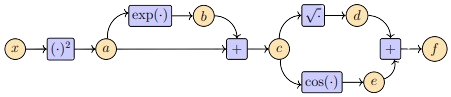
\includegraphics[width=\linewidth, height=2cm, keepaspectratio]{Pictures/maths/AutoDiff-ex5.14.png}
        \end{figure}
    \end{minipage}
    \hfill
    \begin{minipage}{0.39\linewidth}
        \begin{table}[H]
            \centering
            \renewcommand{\arraystretch}{2}
            \begin{tabular}{p{2.5cm} l}
                \textbf{Forward propagation} & \textbf{Backward Propagation} \\ \hline
                
                $a = x^2$ & $\dfrac{\partial a}{\partial x} = 2x$ \\
        
                $b = exp(a) = e^a$ & $\dfrac{\partial b}{\partial a} = b = e^a$\\
        
                $c = a+b$ & $
                \dfrac{\partial c}{\partial a}=1 
                \hspace{0.5cm} 
                \dfrac{\partial c}{\partial b}=1$ \\
        
                $d = \sqrt{c} = c^{0.5}$ & $\dfrac{\partial d}{\partial c}=0.5c^{-0.5} = \dfrac{1}{2\sqrt{c}}$ \\
        
                $e = cos(c)$ & $\dfrac{\partial e}{\partial c} = -sin(c)$\\
        
                $f = d + e$ & $
                \dfrac{\partial f}{\partial d} = 1 
                \hspace{0.5cm} 
                \dfrac{\partial f}{\partial e} = 1$
            \end{tabular}
        \end{table}
    \end{minipage}
\end{table}

\begin{table}[H]
    \renewcommand{\arraystretch}{2}
    \centering
    \begin{tabular}{l l l}
        & \textbf{Calculation} & \textbf{Evaluation} \\
        \hline
    
        $\dfrac{\partial f}{\partial c}$ & 
        $=
            \dfrac{\partial f}{\partial d}
            \dfrac{\partial d}{\partial c}
            +
            \dfrac{\partial f}{\partial e}
            \dfrac{\partial e}{\partial c}
        $ &
        $=
            1\cdot \dfrac{1}{2\sqrt{c}}+
            1\cdot (-sin(c))
        $\\

        $\dfrac{\partial f}{\partial b}$ &
        $=
            \dfrac{\partial f}{\partial c} 
            \dfrac{\partial c}{\partial b}
        $ &
        $
            = \dfrac{\partial f}{\partial c} \cdot 1
        $\\

        $\dfrac{\partial f}{\partial a}$ &
        $=
            \dfrac{\partial f}{\partial b} 
            \dfrac{\partial b}{\partial a}
            +
            \dfrac{\partial f}{\partial c} 
            \dfrac{\partial c}{\partial a}
        $ &
        $
            = \dfrac{\partial f}{\partial b}\exp(a)+
            \dfrac{\partial f}{\partial c}\cdot 1
        $\\

        $\dfrac{\partial f}{\partial x}$ &
        $=
            \dfrac{\partial f}{\partial a}
            \dfrac{\partial a}{\partial x}
        $ &
        $=\dfrac{\partial f}{\partial a}\cdot 2x$
    \end{tabular}
\end{table}










